
% Documentation of IPP
% Martin Benes
% xbenes49
% 2017/2018

\documentclass[10pt,a4paper,titlepage]{article}
\usepackage[english]{babel}
\usepackage[utf8]{inputenc}
\usepackage[margin=80pt]{geometry}


\usepackage{graphicx}   % Import pictures
\usepackage{multicol}

%\newenvironment{changemargin}[2]{%
%\begin{list}{}{%
%\setlength{\topsep}{0pt}%
%\setlength{\leftmargin}{#1}%
%\setlength{\rightmargin}{#2}%
%\setlength{\listparindent}{\parindent}%
%\setlength{\itemindent}{\parindent}%
%\setlength{\parsep}{\parskip}%
%}%
%\item[]}{\end{list}}

\begin{document}

%-----------------------------------------%
%	              DOCUMENT                  %
%-----------------------------------------%

\setcounter{page}{1}
\pagenumbering{arabic}

\begin{center}
\subsection*{Documentation of Project Implementation for IPP 2017/2018}
Name and surname: Martin Benes \\
Login: xbenes49
\end{center}

\paragraph{parse.php}
The script uses a few classes, some of them are used both in {\it parse.php}
and {\it test.php}. Firstly, there is a class hierarchy, used for input-output
operations, defined in {\it io.php}. The abstract class {\it File} implements
the common parts, its specializations {\it FileWriter} and {\it FileReader}
then have the methods, specific for them.

After the start, the program instatiates {\it FileWriter} object to cover
standard input. Afterwards, the {\it Configuration} instance is created.
When the help argument occurs, it raises user-defined {\it HelpException},
which is caught and the program exits successfully. Any other type of Exception
means bad arguments.

The main part of program, compiling IPPcode18 into XML is done in {\it Compiler}.
Its {\it ProcessLine()} method is called repeatly, until it returns false (which
surprisingly means success), in case of error, the exception is raised. The
functionality is basically to split the line to opcode and arguments, and
match, if for given opcode the arguments are valid (count, types). Then using
{\it Instruction} and {\it Argument} classes it is represented and generated
to the output (its {\it FileWriter} is created by {\it Compiler}).

The statistic data, needed by STATP extension, is after the
successful parsing sent to the {\it Configuration}, which generates STATP
output based on the arguments given (it is done notwithstanding it).



\paragraph{interpret.py}
There is a similarity in the design of the {\it Compiler} class from
{\it parse.php} and the {\it Processor} class from {\it interpret.py}.
In addition, the second one processes arguments, raising {\it HelpException},
when the help argument occurs. With one call, the method {\it NextInstuction()}
interprets one instruction. Its usage is semantically same with
{\it ProcessLine()} from {\it Compiler}, described above.

The {\it Processor} creates {\it Reader} instance, that covers the XML library,
so it provides the interface directly connected to the model. Its method
{\it Decode()} returns function, that represents execution of the instruction.
It may raise various types of exception depending on the type of error that
caused them. If the program ends, the {\it ProgramExitException} is raised
but it is caught and the false is returned, so the {\it NextInstruction()} call
cycle is ended regularly. Otherwise the true is returned.






\begin{multicols}{2}
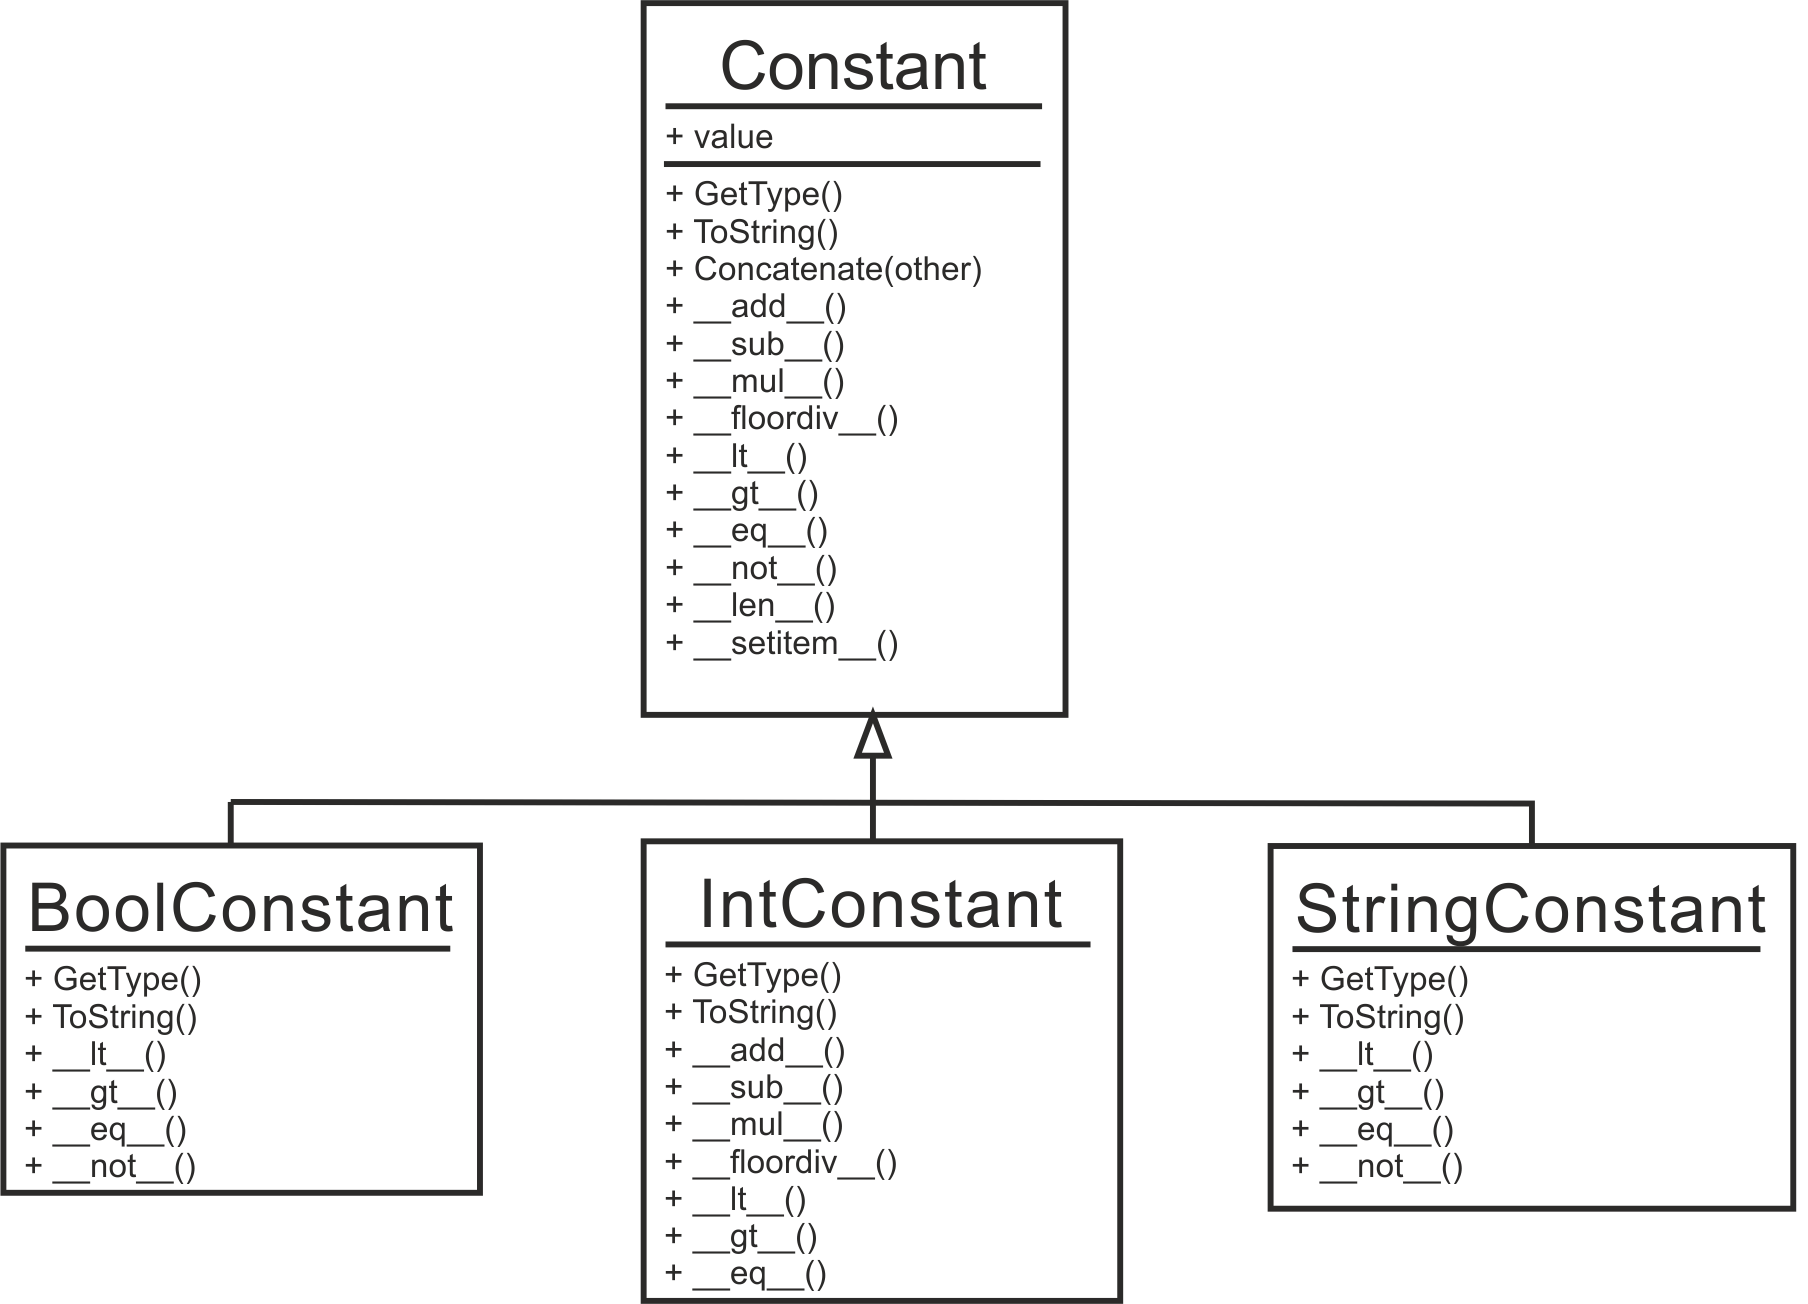
\includegraphics[width=0.45\textwidth]{interpret_constant.png}

\end{multicols}



\paragraph{test.php}
Firstly, it constructs {\it TestSet} and {\it TestConfig} object, that processes
the args and finds the testing files, given to the {\it TestSet} object.

Afterwards, the testing is initiated with {\it Launch()} method of
{\it TestSet} object, receiving {\it Program} object. For each test file,
its method {\it RunTest()} is called. The return value is {\it TestResult}
object, representing the result of testing.

The {\it TestResult} is then analyzed and editted, so the {\it Generator}
object, whom it is given to, could just print the HTML representation with only
a minimum of conditions. It is done at the end of program, printing the
results on standard output in HTML 5 form.

\end{document}
